\begin{figure}[!htbp]
  \centering
  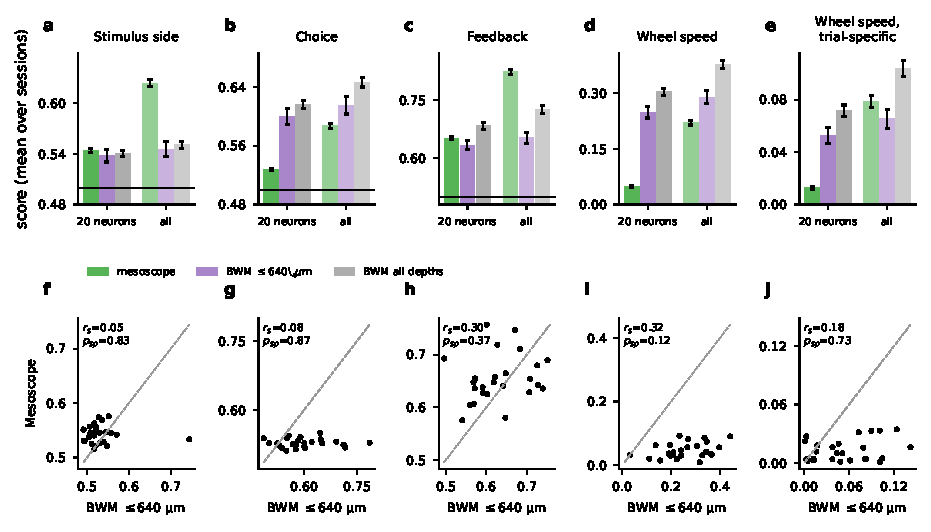
\includegraphics[width=\linewidth,height=0.8\textheight,keepaspectratio]{figures/summary.pdf}
  \caption{Summary of the revised decoding. \textbf{a--e} Mean over sessions ($\pm$ s.e.m.) of each session's mean score over its 1\,mm bins, from 20 random neurons (left, solid) and all neurons (right, light). \textbf{f--j} Per 1\,mm bin, 20 neurons: BWM $\leq$640\,$\mu$m (x) vs mesoscope (y), the 25 bins covered by both; Spearman $r_s$, naive $p$, and $p_{sp}$ against 1000 variogram-matched surrogates of either map (larger $p$ reported). Decoding per session and bin (sessions with $\geq$50 trials and $\geq$20 neurons in the bin), 5-fold cross-validation over trials. Binary variables: L2 logistic regression, balanced accuracy (chance 0.5). Wheel speed in six 0.2\,s bins from $-0.2$ to $1$\,s around movement onset: ridge regression on the activity of the previous, same and next bin (penalty by exact leave-one-trial-out error), cross-validated $R^2$; trial-specific: the same with the mean speed profile of the training trials subtracted, so only trial-to-trial differences in speed count. \textbf{a} Stimulus side, 20 neurons: mesoscope 0.544, BWM $\leq$640\,$\mu$m 0.538, BWM all depths 0.541; all neurons: mesoscope 0.624, BWM $\leq$640\,$\mu$m 0.546, BWM all depths 0.551. \textbf{b} Choice, 20 neurons: mesoscope 0.527, BWM $\leq$640\,$\mu$m 0.600, BWM all depths 0.616; all neurons: mesoscope 0.587, BWM $\leq$640\,$\mu$m 0.615, BWM all depths 0.647. \textbf{c} Feedback, 20 neurons: mesoscope 0.652, BWM $\leq$640\,$\mu$m 0.633, BWM all depths 0.683; all neurons: mesoscope 0.822, BWM $\leq$640\,$\mu$m 0.652, BWM all depths 0.726. \textbf{d} Wheel speed, 20 neurons: mesoscope 0.048, BWM $\leq$640\,$\mu$m 0.248, BWM all depths 0.303; all neurons: mesoscope 0.220, BWM $\leq$640\,$\mu$m 0.289, BWM all depths 0.377. \textbf{e} Wheel speed, trial-specific, 20 neurons: mesoscope 0.013, BWM $\leq$640\,$\mu$m 0.053, BWM all depths 0.072; all neurons: mesoscope 0.079, BWM $\leq$640\,$\mu$m 0.065, BWM all depths 0.104. \textbf{f} Stimulus side: $r_s$ = 0.05, naive $p$ = 0.80, $p_{sp}$ = 0.83. \textbf{g} Choice: $r_s$ = 0.08, naive $p$ = 0.69, $p_{sp}$ = 0.87. \textbf{h} Feedback: $r_s$ = 0.30, naive $p$ = 0.15, $p_{sp}$ = 0.37. \textbf{i} Wheel speed: $r_s$ = 0.32, naive $p$ = 0.11, $p_{sp}$ = 0.12. \textbf{j} Wheel speed, trial-specific: $r_s$ = 0.18, naive $p$ = 0.38, $p_{sp}$ = 0.73.}
  \label{fig:summary}
\end{figure}
